\section{实验结果与分析}

\subsection{实验过程与结果}

\begin{frame}
    \frametitle{实验环境}

    \begin{itemize}
        \item 操作系统:Arch Linux
        \item Golang 工具链:版本 1.20.4,Arch 软件包仓库版本 \texttt{go 2:1.20.4-1};
        \item 处理器:AMD Ryzen 9 4900HS (16) @ 3.000GHz,插入电源;
        \item 内存:16 GB,以及 32 GB 的 Linux 交换空间; 
        \item 安全参数:
        \begin{itemize}
            \item CKKS: PQ12QP109
            \item ECDSA: NIST P-224
        \end{itemize}
    \end{itemize}

\end{frame}

\begin{frame}
    \frametitle{测试描述}

    \begin{itemize}
        \item 客户端:通过 Golang 工具链自带的测试框架,进行相应函数和功能的集成测试和性能评估;\newline 测试内容包括了生成交易的正确性和时间开销、和服务端交互的时间开销等
        \begin{itemize}
            \item 以默认参数执行测试:\texttt{go test -v ./internal/{clientlib,serverlib}}
            \item 以默认参数执行性能测试:\texttt{go test -bench . ./internal/{clientlib,serverlib}}
        \end{itemize}
        \item 服务端:对服务端的测试大部分被包括在了客户端测试中的服务端交互部分,少部分函数单独写了测试和 Benchmark;
    \end{itemize}

\end{frame}

\begin{frame}
    \frametitle{实验结果记录 - Benchmark 截图}

    \begin{figure}
        \centering
        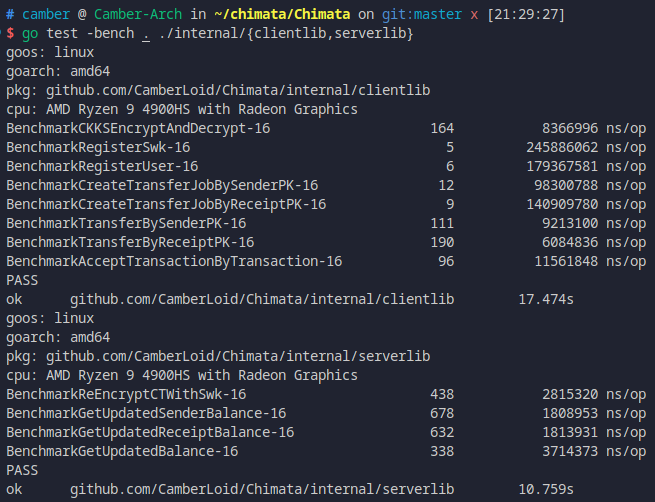
\includegraphics[width=0.8\linewidth]{figures/Bench_Overall.png}
        \caption{Benchmark 截图}
    \end{figure}

\end{frame}

\subsection{实验结果分析}
 
\begin{frame}
    \frametitle{时间开销分析}

    对时间开销的实验数据收集后,汇总如下图:

    \begin{table}[h]
        \begin{tabular}{|l|c|c|c|c|}
            \hline
            类别 & 单笔交易 & 加解密与重加密 & 密态余额更新 & 数据库操作 \\
            \hline
            平均消耗时间 & 105 ms & 15 ms & 4.5 ms & 75.5 ms \\ 
            \hline
            百分比 & 100.0\% & 14.2\% & 4.3\% & 71.9\% \\
            \hline
        \end{tabular}
        \caption{各部分时间开销与单笔交易开销的关系}
    \end{table}

    \begin{itemize}
        \item CKKS 方案相关函数:在指定的安全参数下表现优秀,约 20ms 每笔交易;
        \item 数据库:主要时间开销,有较大优化空间。
        \item 其他:网络交互处理、签名验证等
    \end{itemize}

    %综合上述测试结果,服务端对单笔交易两个不同的方法的平均处理和返回时间约为 105 ms,其中 CKKS 方案的密码学相关函数占比约为 20\%,可以认为在选择的安全参数下,本文的同态加密核心部分工作性能良好。而 CKKS 方案的密码学函数以外的时间开销以数据库操作为主,占据了单笔交易的大部分处理时间,约为 70\%,未来的优化方向可以从这方面入手。其他开销约占比 10\%,包括了网络交互开销和签名验证开销等。

\end{frame}

\begin{frame}
    \frametitle{空间开销分析}

    服务端在处理交易信息后,其存储的密文的数据库大小,即服务端的空间开销进行评估。对实验结果进行收集后绘制如下图:

    \begin{figure}[h]
        \centering
        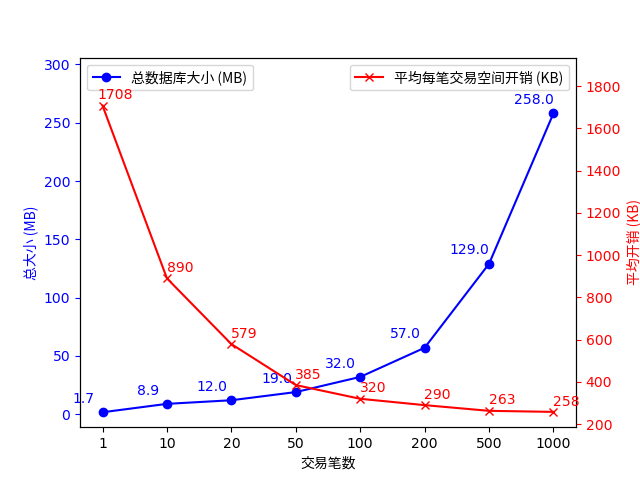
\includegraphics[width=0.8\linewidth]{./figures/Bench_DatabaseSize.png}
        \caption{交易方案的空间开销测试数据}
    \end{figure}

\end{frame}


\begin{frame}
    \frametitle{空间开销分析 - Cont}

    \begin{itemize}
        \item 当交易笔数为 1000 时的约 258 KB 每笔交易,推算,每 1 GB 空间可以存储约 4000 笔交易信息;
        \item 考虑到目前计算机存储成本越来越低,可以认为本文所提出的服务端实现具有较高的空间效率,具有可实现性;
        \item 未引入数据压缩算法:可以预期较大的空间效率提升,如 gzip。
    \end{itemize}

\end{frame}
